\documentclass[main.tex]{subfiles}
\begin{document}

\begin{chapquote}{página 65}
	``Counting can become quite subtle, and in this chapter we explore some of its more sophisticated aspects. Our goal is still to answer the question 'How many?' but we introduce mathematical techniques that bypass the actual process of counting individual objects''
\end{chapquote}

\section{Listas}

Uma \textbf{lista} é uma sequência ordenada de objetos. Esses objetos são mantidos entre um par de parênteses e separados por vírgulas. Os objetos dentro de uma lista são chamados de \textbf{entradas}\footnote{Do original, \textbf{entries}}. Já que uma lista é uma sequência ordenada, é evidente que a ordem dos seus elementos é suficiente para distinguir listas que contenham os mesmo objetos.

$$ (a,b,c) \neq (c,b,a) $$

\textbf{Comentário}: Também é comum escrever uma lista sem os parênteses e as vírgulas. Esse formato de escrita se chama \textbf{string}. Nesse caso $(a,b,c)$ é a mesma coisa de $abc$. Essa outra maneira só é usada quando não há risco de confusão entre as entradas da lista. Mantenha essas duas formas de escrita como padrão na sua mente.
\\~\\
Como já vimos conjuntos no capítulo 01, podemos usá-los para comparação. No caso dos conjuntos a ordem dos elementos não importa na comparação. Ou seja, $\{a,b,c\} = \{c,b,a\}$. Já vimos acima que essa propriedade não é mantida nas listas. 
\\~\\
Diferentemente dos conjuntos, uma lista pode ter entradas repetidas sem nenhum problema. A lista $(a,a,a,a,b)$, por exemplo, é perfeitamente aceitável.
\\~\\
Tal qual a cardinalidade dos conjuntos, nós contamos quantas entradas existem em uma lista. Chamamos essa medida de \textbf{comprimento}. A lista $(a,a,a,a,b)$ possui um comprimento de 5.
\\~\\
\textbf{Regra}: Duas listas são \textbf{iguais} se possuírem exatamente as mesmas entradas nas mesmas posições, ou seja, também possuem o mesmo comprimento.
\\~\\
Só existe uma lista cujo comprimento é igual a zero. Denominamos essa lista de \textbf{lista vazia}. Denotada por $()$.\footnote{Sim, lembra muito o conceito de conjunto vazio.}

\section{O Princípio da Multiplicação}

Existem muitos problemas práticos que envolvem a contagem do número possível de listas que satisfazem uma determinada condição ou propriedade. Por causa disso, vamos aprender uma maneira de trabalharmos essa questão sem precisar ficar escrevendo todas as listas possíveis antes de contar os resultados.

\begin{fact}[Princípio da Multiplicação]
Suponha que em uma lista de comprimento $n$ exista $a_1$ escolhas possíveis para a primeira entrada, $a_2$ escolhas possíveis para a segunda entrada, $a_3$ escolhas possíveis para a terceira entrada e etc. Então, o total de listas diferentes que podem ser geradas por essas entradas será igual ao produto entre $a_1 \times a_2 \times a_3 \times \dots \times a_n$. 
\end{fact}

\textbf{Dica}: Nas páginas 67 e 68 do livro, o professor coloca dois exemplos que tornarão esse conceito abaixo bem mais entendível. Se você não entender como esse fato é evidente, dá uma olhada no livro e volta aqui.
\\~\\
Embora no livro não seja dada uma demonstração desse princípio. Achamos que a provadessa afirmação é útil para exercitarmos os conceitos que vimos até a gora. Não se preocupe se você não conseguir entender essa demonstração agora. Volte quando estiver mais adiantado no curso e tente novamente.

\begin{demonstration}[Princípio da Multiplicação\footnote{A ideia da primeira parte da demonstração para $m \leq 2$ veio desse livro: JOHNSTON, William; MCALLISTER, Alex. A transition to advanced mathematics: a survey course. OUP USA, 2009. p. 365. Pra segunda parte, onde $m > 2$, a inspiração veio desse link do 
\href{https://math.stackexchange.com/questions/3053969/using-induction-to-prove-the-multiplication-rule}{StackExchange.}}]

Começaremos com a proposição $P(m)$: "Se existirem $m \in \mathbb{N}$ conjuntos $A_i$ com $n_i$ elementos em cada conjunto onde $i \in \{1,2,\dots,m\}$. O Cardinal do produto cartesiano de todos os $m$ conjuntos será igual à multiplicação de todos os $m$ cardinais $| A_i|$, ou seja, $ |A_1 \times A_2 \times \dots \times A_m | = \prod_{i = 1}^{m}\limits | A_i | $"\footnote{O nome desse símbolo é \href{https://en.wikipedia.org/wiki/Multiplication\#Product_of_a_sequence}{"Produtório"}}.
\\~\\
Essa proposição é equivalente ao enunciado do princípio da multiplicação.\footnote{Você consegue ver essa equivalência?}
\\~\\
Quando $m = 1$, temos apenas o conjunto $A_1$ que possui $n_1$ elementos. Portanto, o cardinal de todos os $m = 1$ conjuntos é igual ao cardinal do único conjunto ($|A_m| = |A_1|$). Com isso, vemos que $P(1)$ é verdadeira.
\\~\\
$P(2)$: "Se $A_1$ e $A_2$ são conjuntos finitos onde $A_1$ contém $n_1$ elementos e $A_2$ contém $n_2$ elementos, então, o conjunto $A_1 \times A_2$ possui $n_1 \cdot n_2$ elementos".
\\~\\
A demonstração dessa proposição é simples. Para cada um dos $n_1$ elementos $a \in A_1$ na primeira coordenada do par ordenado $(a,b) \in A_1 \times A_2$, existem exatamente $n_2$ elementos $b \in A_2$. Uma vez que existem $n_1$ elementos em $A_1$ que podem ser essa primeira coordenada do par ordenado $(a,b)$, então, existem ao todo $n_1 \cdot n_2$ possíveis pares ordenados no produto cartesiano $A_1 \times A_2$.
\\~\\
Agora vamos fazer uma pequena adaptação nessa demonstração para qualquer quantidade de conjuntos, ou seja, para qualquer $P(m)$ cujo $m > 2$.
\\~\\
Suponha que agora temos 3 conjuntos: $A_1$, $A_2$ e $A_3$. Para podermos demonstrar $P(3)$: "Se $A_1 \times A_2 \times A_3$, então o cardinal será  $n_1 \cdot n_2 \cdot n_3$"\  só precisamos da seguinte linha de pensamento: Podemos definir um novo conjunto $B = A_1 \times A_2$. Desse modo, podemos reescrever o cardinal anterior como $B \times A_3$. Essa reescrita possui apenas dois elementos. Portanto, podemos usar a proposição já demonstrada $P(2)$ sem nenhum prejuízo.
\\~\\
Aplicando esse mesmo procedimento para qualquer $m > 2$ fica demonstrado que o cardinal de quaisquer conjuntos $A_i$ para qualquer $i \in \{1,2,\dots,m\}$ será a multiplicação do cardinal dos conjuntos $A_i$. Aplicando a equivalência da proposição $P(m)$ com o princípio da multiplicação, finalizamos a demonstração. $\blacksquare$
\end{demonstration}

Existem dois tipos de problemas que envolvem contagem de listas: Problemas que possuem entradas repetidas (como a construção de placas de carros, números de telefone e etc) e Problemas que não permitem entradas repetidas (como ordenar pessoas em uma fila). Nós podemos chamar as listas do segundo tipo de problema de \textbf{listas não repetitivas}.
\\~\\
Usando o princípio da multiplicação você é capaz de resolver todos os problemas envolvendo contagens de listas (com e sem repetição) sem precisar ficar escrevendo as soluções possíveis, ao invés disso, você só precisa interpretar as opções de entradas na lista e usar a multiplicação.
\\~\\
\textbf{Dica}: Tente fazer os exemplos 3.1, 3.2 e 3.3 da página 69 até a 72.

\section{Os Princípios da Adição e Subtração}

Vamos ver mais dois princípios de contagem. Você já está familiarizado com eles mas agora definiremos esses princípios usando a linguagem dos conjuntos.

\begin{fact}[Princípio da Adição]
Suponha que um conjunto finito $X$ pode ser decomposto na união $X = \bigcup_{i = 1}^{n}\limits X_i$ onde $ X_i \cap X_j = \emptyset \ \forall \ i \neq j$. Então, $|X| = \sum_{i = 1}^{n}\limits |X_i|$.
\end{fact}

Calma. Não é difícil de entender. O que estamos dizendo ai é: "Se $X$ é um conjunto formado por $n$ outros conjuntos menores de modo que nenhum desses conjuntos possui interseção entre si. Então, o cardinal de $X$ será a soma dos cardinais de todos os $n$ subconjuntos. A única coise que pode assustar nessa notação é o sigma ($\sum$) para denominar somatório.\footnote{Já vimos essa notação no capítulo 01.}
\\~\\
\textbf{Dica}: Veja os exemplos 3.5 e 3.6 na página 75 para ter uma ideia da aplicação desses conceitos na prática.

\begin{fact}[Princípio da Subtração]
Se $X$ é um subconjunto de um conjunto finito $U$, então $|\overline{X}| = |U| - |X|$. Ou seja, se $X \subseteq U$, então $|U - X| = |U| - |X|$.
\end{fact}

Existem situações onde é mais fácil contar o total de um conjunto maior, e retirar uma parte desse total que não queremos, do que contar diretamente a parte desejada. A primeira vista pode parecer um pouco confuso mas a ideia é simples: Usamos esse método para computar o que sobra após a retirada de algumas opções.
\\~\\
\textbf{Dica}: Leia o exemplo 3.7 novamente. A gente usa exatamente essa abordagem pra chegar no resultado.

\section{Fatoriais e Permutações}
O processo de contagem para listas não repetitivas de tamanho $n$ é tão comum que criamos um conceito especial para lidar com esse tipo de problema. O conceito em questão é o \textbf{Fatorial} ($n!$). Antes de formalizarmos, observe o quadro abaixo.
\\~\\
\begin{center}
\begin{tabular}{ | c | c | c | c | }
 \hline
 n & Elementos & Listas não repetidas de tamanho $n$ & $n!$ \\ 
 \hline
 0 & $\{\}$ & $()$ & 1 \\
 1 & $\{a\}$ & $(a)$ & 1 \\
 2 & $\{a,b\}$ & $(a,b), (b,a)$ & 2 \\
 3 & $\{a,b,c\}$ & $(a,b,c),(a,c,b),(b,a,c),(b,c,a),(c,a,b),(c,b,a) $ & 6 \\
 \vdots & \vdots & \vdots & \vdots \\
\end{tabular}
\end{center}

Consegue ver como a quantidade de listas não repetitivas cresce rápido com apenas o incremento de 1 elemento no exemplo?. O número da última coluna é obtido pela aplicação do princípio da multiplicação. Nós chamamos esse número de \textbf{Fatorial} de $n$. Seu símbolo é esse ponto de exclamação ao lado direito do número "$n!$"\footnote{Lemos como "$n$ fatorial".}.

\begin{definition}[Fatorial]
Se $n$ é um número inteiro não negativo, então $n!$ será o número de listas de tamanho $n$ que podem ser formadas com $n$ símbolos, sem repetições. Desse modo, temos que $0! = 1, 1! = 1$. Para qualquer $n > 1$, então $n! = n \times (n - 1) \times (n - 2) \times \dots \times 3 \times 2 \times 1 $.
\end{definition}

\textbf{Dica}: O exemplo 3.8 na página 79 é ótimo pra exercitar esses conceitos vistos até agora.
\\~\\
Outro conceito importante\footnote{Que eu aposto que você viu no ensino médio e achou que nunca ia usar.} é o conceito de \textbf{Permutação}. Quando computamos um fatorial, estamos, na verdade, contando a quantidade de listas de comprimento $n$ que podem ser geradas a partir da mudança da ordem dos $n$ elementos.
\\~\\
\textbf{Comentário}: Guarde na memória que o \textbf{Fatorial} conta o número de \textbf{Permutações} possíveis para $n$ elementos via aplicação do \textbf{princípio da multiplicação}.
\\~\\
Agora vamos estender um pouco mais esse pensamento. Se temos um total de $n$ elementos. Uma permutação é uma lista de comprimento $n$. Mas e se não quisermos usar todos os elementos disponíveis na composição dessas listas? Para isso o autor usa o conceito de \textbf{k-permutação}\footnote{Do original: k-permutation.} (aqui no Brasil você viu esse conceito pelo nome de \textbf{Arranjo}). Uma k-permutação será uma lista de tamanho $k$ formada por um subconjunto dos $n$ elementos anteriores.
\\~\\
Para facilitar (ou não) a nossa vida, vamos definir uma notação para situações onde queremos fazer permutações de comprimento $k$ de um conjunto qualquer de tamanho $n$. Escreveremos $P(n,k)$ para denotar essa situação.\footnote{Perceba que se $k = n$ teremos que $P(n,k) = n!$. Não tem problema nenhum se não entender. Vamo bater um papo no \href{https://twitter.com/bruno_ruas2}{twitter} que eu te explico com mais calma.} 
\\~\\
Para o caso onde $k = 0$ só precisamos pensar em quantas listas de comprimento $0$ conseguiríamos fazer a partir de um conjunto com $n$ elementos. Isso mesmo, só temos uma lista possível - a lista vazia $()$. 
\\~\\
Para todos os casos onde $k \leq n$ podemos calcular o número de k-permutações usando o princípio da multiplicação. Na página 81 tem uns exemplos sobre isso.
\\~\\
Nos casos onde $k > n$ seria como responder algo parecido com: "Quantas lista de 4 elementos podemos fazer com 3 números". A resposta é "zero listas".
\\~\\
De modo mais geral, via princípio da multiplicação, temos que para a primeira entrada da lista de comprimento $k$ temos sempre $(n)$ opções. Para a segunda entrada, teremos $(n - 1)$ opções. Para a terceira entrada teremos $(n - 2)$ opções. Podemos ver claramente um padrão se formando. Podemos definir que o número de escolhas para a posição $i \in \{1,2,\dots,k\}$ será $(n - i + 1)$\footnote{Por exemplo: \\ $i = 1 \implies (n - 1 + 1) = (n)$ opções \\ $i = 2 \implies (n - 2 + 1) = (n - 1)$ opções}. Quando $i = k$ teremos então $(n - k + 1)$ opções.
\\~\\
Com isso podemos chegar em uma equação:
\begin{center}
$ P(n,k) = n . (n - 1) . (n - 2) \dots (n - k + 1) $
\end{center}

Podemos ainda transformar essa relação em outra equação. Primeiro pensemos no que essa parte direta da equação acima quer dizer. Ela se parece com a fórmula do fatorial de $n$ mas com a diferença de "parar" \ em $(n - k + 1)$. Para recuperar o formato do fatorial podemos multiplicar a equação acima por $ (n - k) . (n - k - 1) \dots 3 . 2 . 1 $ e dividir pela mesma expressão.

\begin{center}
\small $ P(n,k) = \dfrac{n . (n - 1) . (n - 2) \dots (n - k + 1) . (n - k) . (n - k - 1) \dots 3 . 2 . 1}{(n - k) . (n - k - 1) \dots 3 . 2 . 1} = \dfrac{n!}{(n-k)!}$
\end{center}

Depois de todas essas manipulações, podemos formalizar o conceito de k-permutações.

\begin{fact}[K-Permutações ou Arranjos]
Uma \textbf{k-permutação} ou \textbf{Arranjo} de um conjunto com $n$ elementos é uma lista de comprimento $k$ feita com elementos desse conjunto. Informalmente, podemos pensar nessa lista como fruto do "rearranjo"\ dos elementos desse conjunto.
\\~\\
O número de k-permutações de um conjunto com $n$ elementos é denotado por $P(n,k)$ e é dado por:\\
\begin{center}
$ P(n,k) = n . (n - 1) . (n - 2) \dots (n - k + 1) $
\end{center}

Se $0 \leq k \leq n$, então temos que:\\
\begin{center}
 $ P(n,k) = \dfrac{n!}{(n - k)!} $
\end{center}
\end{fact}


\section{Contando Subconjuntos}

Até agora, vimos quantas listas de tamanho $k$ podemos fazer com todos os $n$ elementos de um conjunto qualquer. Agora, vamos expandir essa linha de pensamento para um tópico correlato: "Quantos subconjuntos podem ser feitos se selecionarmos $k$ elementos de um conjunto de $n$ elementos?". 
\\~\\
Algum leitor de pensamento rápido pode pensar que se trata exatamente do mesmo problema. Contudo, não é o caso. A diferença reside nas propriedades de uma \textbf{lista} e de um \textbf{conjunto}.
\\~\\
Uma lista leva em consideração a ordem dos seus elementos, ou seja, $(a,b) \neq (b,a)$ enquanto os conjuntos só se preocupam com os valores dos seus elementos $\{a,b\} = \{b,a\}$. Para prosseguirmos vamos definir essa tarefa de "contar subconjuntos" \ usando uma notação.
\\~\\
\textbf{Comentário}: Estranhamente, o professor não dá um nome para o conceito que ele vai definir agora. Nós achamos por bem usar o nome que os materiais didáticos do Brasil utilizam.

\begin{definition}[Combinação]
Se $k,n \in \mathbb{Z}$, então $n \choose k$, ou alternativamente, $C(n,k)$, denota o número de subconjuntos que podem ser feitos escolhendo $k$ elementos de um conjunto com $n$ elementos. Lemos $n \choose k$ como "de $n$ escolhemos $k$".
\end{definition}

\textbf{Comentário}: Aqui já temos algo para guardar na mente. Se tivermos um conjunto com $n$ elementos, sempre será verdade que $P(n,k) \geqslant $ $n \choose k$ ou, na outra notação, $P(n,k) \geqslant C(n,k)$. Ou seja, sempre será verdade que os arranjos serão maiores ou iguais que as combinações para quaisquer $n$ e $k$.
\\~\\
Já definimos o que queremos dizer quando escrevemos $n \choose k$ e sabemos bem qual problema queremos responder com essa notação nova. Precisamos de uma fórmula que nos permita encontrar a solução de quaisquer valores de $n$ e $k$. Para tanto, vamos começar com um exemplo prático: $5 \choose 3$.
\\~\\
Nós já sabemos que se fossem listas ao invés de subconjuntos, teríamos $P(5,3) = \frac{5!}{(5 - 3)!} = 60$ listas possíveis. Também já sabemos que $P(5,3) \geqslant $ $5 \choose 3$.
\\~\\
O pensamento para chegarmos no nosso resultado é o seguinte: "Quantas listas podemos formar com cada subconjunto de 3 elementos?". A resposta é obtida pela aplicação do princípio da multiplicação. Isso nos dá $3! = 6$ listas possíveis para cada subconjunto de 3 elementos.
\\~\\
Agora que sabemos que teremos 6 listas para cada subconjunto formado por 3 elementos e também sabemos que podemos formar um total de 60 listas diferentes. Basta dividirmos as 60 listas por 6 que chegaremos no total de 10 subconjuntos possíveis.
\\~\\
\textbf{Dica}: Na página 89 o professor monta uma tabela com todos os subconjuntos e as listas que falamos aqui.
\\~\\
De maneira mais abstrata, o que fizemos foi dividir a k-permutação $P(5,3)$ por $3!$. Ou seja, podemos saber quantos subconjuntos de tamanho $k$ podem ser formados com $n$ elementos pela equação abaixo.

\begin{fact}[Cálculo das Combinações]
Se $0 \leq k \leq n$, então:
\begin{center}
 \Large ${n \choose k} = \frac{n!}{k!(n-k)!}$
\end{center}
\end{fact}

Se $k > n$ então $n \choose k$ $= 0$. Seria como perguntar algo como "quantos subconjuntos de 5 elementos podemos fazer com 3 elementos? Isso mesmo, zero conjuntos.

\section{O Triângulo de Pascal e O Teorema Binomial}
Até aqui você é capaz de resolver qualquer problema que envolva contagens de listas e subconjuntos seja usando todos os valores disponíveis ou apenas uma parte deles. Mas uma coisa interessante da matemática é que alguns padrões surgem a medida que se criam novos conceitos.
\\~\\
Um desses padrões foi descoberto em vários países em épocas diferentes, mas o nome que usaremos é atribuído ao matemático francês Blaise Pascal e é denominado \href{https://pt.wikipedia.org/wiki/Tri\%C3\%A2ngulo_de_Pascal}{Triângulo de Pascal}.
\\
A relação é simples:
\\
$$ {n+1 \choose k} = {n \choose k-1} + {n \choose k} $$
\\
Ou seja, o número de subconjuntos que podemos formar com a adição de apenas 1 elemento no universo de opções é igual à soma dos totais de subconjuntos de tamanho $k-1$ das opções originais com a quantidade de subconjuntos de tamanho $k$ das $n$ opções originais. Parece um pouco chato todo esse papo, mas se certifique que está acompanhando.
\\~\\
Para verificar se o triângulo de Pascal é verdadeiro, vamos começar quebrando a equação e desenvolvendo suas formas completas:
$$ {n+1 \choose k} = \frac{(n+1)!}{k!(n+1-k)!}$$
\\
e
\\
$${n \choose k-1} + {n \choose k} = \frac{n!}{(k-1)![n-(k-1)]!} + \frac{n!}{k!(n-k)!}$$
\\
Não se assuste, foram apenas pequenas alterações feitas na formulação clássica de $n \choose k$. Escreva em um papel para se certificar que entendeu.
\\~\\
A próxima parte é bem feia e pode assustar mas é simplesmente uma soma de frações comum do estilo $\frac{a}{b} + \frac{c}{d} = \frac{ad+cb}{bd}$:
$${n+1 \choose k} = \frac{n!k!(n-k)!}{k!(n-k)!(k-1)!(n-k+1)} + \frac{n!(n-k+1)!}{k!(n-k)!(k-1)!(n-k+1)!}$$
$${n+1 \choose k} = \frac{n!k!(n-k)! + n!(n-k+1)!}{k!(n-k)!(k-1)!(n-k+1)!}$$
\\
Para ficar mais fácil de visualizar vou abrir os fatoriais $k!$ e $(n-k+1)!$:
$${n+1 \choose k} = \frac{n!k(k-1)!(n-k)! + n!(k-1)!(n-k+1)(n-k)!}{k!(n-k)!(k-1)!(n-k+1)!}$$
\\
Perceba que temos $(k-1)!(n-k)!$ em ambas as parcelas da soma podemos transformar isso em:
\\
$${n+1 \choose k} = \frac{(n-k)!(k-1)![n!k+n!(n-k+1)]}{(k-1)!(n-k+1)!k!(n-k)!} = \frac{n!k + n!(n-k+1)}{k!(n-k+1)!}$$
\\
Opa! Chegamos em um ponto interessante, temos ambos os divisores iguais, agora resta mostrar que os dividendos são iguais. Para que fique mais limpo trabalharei com os dividendos separadamente. Agora só temos que provar essa pequena igualdade:
\\
$$ (n + 1)! = n!k + n!(n - k + 1) $$
\\
Primeiramente relembremos:
\\
$$ (n+1)! = (n+1)\underbrace{(n)(n-1)...3.2.1}_{ \ Isso \ aqui \ é \ igual \ a \ n!} $$
\\
Então podemos simplificar a equação restante como
\\
$$ (n+1)n! = n!k + n!(n-k+1) $$
$$ (n+1)\cancel{n!} = \cancel{n!}k + \cancel{n!}(n-k+1) $$
$$ (n+1) = k + n - k + 1 $$
$$ (n+1) = \cancel{k} + n\cancel{-k}+1 $$
$$ (n+1) = (n+1) $$
\\
Com divisores e dividendos iguais concluímos que:
$$ {n+1 \choose k} = {n \choose k-1} + {n \choose k} \blacksquare$$
\\
Tendo mostrado que essa propriedade é verdadeira podemos ver como o Triângulo de Pascal é verdadeiro.\footnote{Você com certeza viu isso, mas em formato de pirâmide, aqui é um Triângulo Retângulo de Pascal.}
\\
\begin{center}
\begin{tabular}{ | c | c c c c c c c c | }
\hline
  $n/k$ &$0$& $1$ & $2$ & $3$ & $4$ & $5$ & $\cdots$ & $k$ \\
\hline
$0$     & \tiny $0 \choose 0$ &               &               &               &               &              &         & \\
$1$     & \tiny $1 \choose 0$ & \tiny $1 \choose 1$ &               &               &               &              &         & \\
$2$     & \tiny $2 \choose 0$ & \tiny $2 \choose 1$ & \tiny $2 \choose 2$ &               &               &              &         & \\
$3$     & \tiny $3 \choose 0$ & \tiny $3 \choose 1$ & \tiny $3 \choose 2$ & \tiny $3 \choose 3$ &               &              &         & \\
$4$     & \tiny $4 \choose 0$ & \tiny $4 \choose 1$ & \tiny $4 \choose 2$ & \tiny $4 \choose 3$ & \tiny $4 \choose 4$ &              &         & \\
$5$     & \tiny $5 \choose 0$ & \tiny $5 \choose 1$ & \tiny $5 \choose 2$ & \tiny $5 \choose 3$ & \tiny $5 \choose 4$ & \tiny $5 \choose 5$&         & \\
$\vdots$&\tiny $\vdots$       &\tiny $\vdots$       &\tiny $\vdots$       &\tiny $\vdots$       &\tiny $\vdots$       &\tiny $\vdots$      &\tiny $\ddots$ & \\
$n$     & \tiny $n \choose 0$ & \tiny $n \choose 1$ & \tiny $n \choose 2$ & \tiny $n \choose 3$ & \tiny $n \choose 4$ & \tiny $n \choose 5$&\tiny $\cdots$ & \tiny $n \choose k$\\
\hline

\end{tabular}
\end{center}
Fazendo os devidos cálculos pela aplicação para todos os casos ${n \choose k}$ teremos:
\begin{center}
\begin{tabular}{ | c | c c c c c c c | }
\hline
 $n/k$ &$0$& $1$ & $2$ & $3$ & $4$ & $5$ & $\cdots$  \\
\hline
$0$     & $1$ &     &        &      &     &     & \\
$1$     & $1$ & $1$ &        &      &     &     & \\
$2$     & $1$ & $2$ & $1$    &      &     &     & \\
$3$     & $1$ & $3$ & $3$    & $1$  &     &     & \\
$4$     & $1$ & $4$ & $6$    & $4$  & $1$ &     & \\
$5$     & $1$ & $5$ & $10$   & $10$ & $5$ & $1$ & \\
$\vdots$&     &     &$\vdots$&      &     &     & $\ddots$ 
\end{tabular}
\end{center}

Para prosseguirmos, o professor Hammack usa os exercícios 3.5.13 e 3.5.14 como ferramentas para expor algumas implicações do triângulo de Pascal.
\\~\\
\textbf{Exercício 3.5.13}: Suponha que $n,k \in \mathbb{Z}$ e $0 \leq k \leq n$. De posse da fórmula da combinação \tiny ${n \choose k} = \frac{n!}{k!(n-k)!}$ \normalsize , demonstre que \tiny $ {n \choose k} = {n \choose {n-k}} $ \normalsize.
\\~\\
A resposta para essa questão está no solucionário do próprio livro. Assumindo que $ n,k \in \mathbb{Z} $ e $ 0 \leq k \leq n $, aplicando o conceito das combinações podemos ver que \tiny $ {n \choose n - k} = \frac{n!}{(n-k)![n-(n-k)]!} = \frac{n!}{(n-k)![n-n+k)]!} = \frac{n!}{(n-k)![\cancel{n-n}+k)]!} = \frac{n!}{(n-k)!k!} = {n \choose k} \blacksquare$ \normalsize
\\~\\
\textbf{Exercício 3.5.14}: Suponha que $n,k \in \mathbb{Z}$ e $0 \leq k \leq n$. Usando apenas a definição de combinação da página 31 (sem usar a fórmula), demonstre que \tiny $ {n \choose k} = {n \choose {n-k}} $ \normalsize.  
\\~\\
Para responder essa questão nós vamos ter que abordar 3 casos possíveis. Quando temos $ k = n $, estamos dizendo que queremos saber quantos subconjuntos de tamanho $n$ podemos fazer com $n$ elementos, cuja resposta é claramente 1. Quando temos $ k = 0 $, só temos 1 subconjunto possível, que é o conjunto vazio $\emptyset$. Ou seja, $\{k = 0 \ \lor \  k = n\} \implies {n \choose k} = {n \choose n - k}$.\footnote{Se você leu o capítulo 02, você entendeu o que a gente quis dizer aqui.}
\\~\\
Agora teremos que trabalhar com os casos onde $0 < k < n$. Dentro dessa situação, temos o caso onde $k = n/2$. Nesse caso, é simples ver que ${n \choose k} = {n \choose \frac{n}{2}} = {n \choose n - \frac{n}{2}} = {n \choose \frac{n}{2}} = {n \choose n - k}$. Agora que já eliminamos todos os casos mais evidentes, precisamos desenvolver uma lógica que contemple todos os demais.
\\~\\
Primeiro vamos pensar num conjunto qualquer $N$. Como estamos contando subconjuntos, se $N$ possuir elementos repetidos, isso não nos afeta visto que um conjunto não leva em consideração a ordem nem elementos repetidos. Para nos certificarmos, vamos criar um subconjunto $N^* = \{n \in N : n_k \neq n_w \ \forall \  k \neq w \}$. Esse conjunto $N^*$ não tem nenhum elemento repetido. Primeiro vamos contar todos os subconjuntos de tamanho $k$ de $N^*$. Cada subconjunto $k_i \subseteq N^*$ será do tipo $\{n_1,n_2,n_3,...,n_k\}$. Uma vez que formamos um conjunto $k_i$ ainda teremos $n - k$ elementos "sobrando"\ para criarmos novos subconjuntos. Desse modo, teremos um total de $k(n-k)$ possibilidades. Do outro lado do problema, vamos pensar no caso para os subconjuntos de tamanho $(n-k)$. Eles serão do tipo $\{n_1,n_2,...,n_{n-k}\}$. Similarmente, para cada subconjunto com $(n-k)$ elementos, teremos $n-(n-k)=n-n+k=k$ elementos "sobrando"\ para construirmos novos subconjuntos. O que também nos dá um total de $k(n-k)$ subconjuntos possíveis. Como temos o mesmo número de possibilidades, fica demonstrada a simetria entre ${n \choose k}$ e ${n \choose n-k}$ de acordo com o enunciado da questão. $\blacksquare$
\\~\\
Com a demonstração dos exercícios 3.4.13 e 3.4.14 nós podemos ver que o triângulo de Pascal possui uma simetria. Começando pelas laterais, as colunas onde $k = 0$ e $k = n$ são sempre iguais a $1$. Mas além dessas, as colunas intermediárias também possuem uma simetria dada por ${n \choose k} = {n \choose n-k}$. Isso quer dizer que as segundas colunas sempre serão iguais às penúltimas. Do mesmo modo, as terceiras colunas sempre serão iguais às antepenúltimas. Nos casos onde o $k$ é ímpar, teremos uma coluna do meio que será a única sem uma repetição do valor.
\\~\\
A partir dessa simetria, os matemáticos perceberam uma relação entre os valores de cada elemento das linhas do triângulo de Pascal com os coeficientes dos binômios do tipo $(a+b)^n$. Esse fato é chamado de \textbf{Teorema Binomial}. Como o nome diz, um \textbf{binômio} é formado por quaisquer dois números (chamados de monômios) $a$ e $b$ relacionados por uma soma.

\pagebreak

Veja só que interessante:
\\~\\
$(a+b)^0 = \textcolor{red}{1}$ \\
$(a+b)^1 = \textcolor{red}{1}a + \textcolor{red}{1}b$ \\
$(a+b)^2 = \textcolor{red}{1}a^2 + \textcolor{red}{2}ab + \textcolor{red}{1}b^2$ \\
$(a+b)^3 = \textcolor{red}{1}a^3 + \textcolor{red}{3}a^2b + \textcolor{red}{3}ab^2 + \textcolor{red}{1}b^3$ \\
$(a+b)^4 = \textcolor{red}{1}a^4 + \textcolor{red}{4}a^3b + \textcolor{red}{6}a^2b^2 + \textcolor{red}{4}ab^3 + \textcolor{red}{1}b^4$ \\
$(a+b)^5 = \textcolor{red}{1}a^5 + \textcolor{red}{5}a^4b + \textcolor{red}{10}a^3b^2 + \textcolor{red}{10}a^2b^3 + \textcolor{red}{5}ab^4 + \textcolor{red}{1}b^5$ \\
$(a+b)^6 = \textcolor{red}{1}a^6 + \textcolor{red}{6}a^5b + \textcolor{red}{15}a^4b^2 + \textcolor{red}{20}a^3b^3 + \textcolor{red}{15}a^2b^4 + \textcolor{red}{6}ab^5 + \textcolor{red}{1}b^6$ \\
$(a+b)^7 = \textcolor{red}{1}a^7 + \textcolor{red}{7}a^6b + \textcolor{red}{21}a^5b^2 + \textcolor{red}{35}a^4b^3 + \textcolor{red}{35}a^3b^4 + \textcolor{red}{21}a^2b^5 + \textcolor{red}{8}ab^6 + \textcolor{red}{1}b^7$  \\~\\
Perceba como os coeficientes em vermelho seguem exatamente o padrão estabelecido pelo triângulo de Pascal. Nós vamos partir dessa constatação para a definição do teorema binomial. Relaxa que a gente vai indo em partes.
\\~\\
Os primeiros e últimos termos do binômio estão a n-ésima potência,\footnote{Deixarei $a^{n-n}$ multiplicando o último termo e $b^{n-n}$ o primeiro, apenas para que o desenvolvimento fique mais claro, afinal, é um número elevado a zero e não mudará nosso resultado} portanto:
$$(a+b)^n = a^nb^{n-n} + \cdots + a^{n-n}b^n $$
\\
Agora veja que o no segundo termo do binômio temos $a^{n-1}b^1$ e no penúltimo $a^1b^{n-1}$
\\
$$(a+b)^n = a^nb^{n-n} + a^{n-1}b^1 + \cdots + a^1b^{n-1} + a^{n-n}b^n $$
\\
Por fim, falta apenas incluir os coeficientes, que como dito antes, seguirão por padrão a k-ésima entrada da n-ésima linha do Triângulo de Pascal:
\\
$$(a+b)^n = {n \choose 0}a^nb^{n-n} + {n \choose 1}a^{n-1}b^1 + \cdots + {n \choose n-1}a^1b^{n-1} + {n \choose n}a^{n-n}b^n $$
\\
Um fator importante para a notação mais limpa é que $a$ está sempre elevado a $n$ subtraído a k-ésima entrada, e $b$ está sempre elevado a k-ésima potência.
\\~\\
Pronto. Com isso já conseguimos definir nosso teorema.

\begin{theorem}[Teorema Binomial]
Se $n$ é um inteiro não negativo, então:
$$(a+b)^n = {n \choose 0}a^{n-0}b^{0} + {n \choose 1}a^{n-1}b^1 + \cdots + {n \choose n-1}a^1b^{k-1} + {n \choose n}a^{0}b^k $$
\\
Que também pode ser expresso como:
$$(a+b)^n = \sum\limits_{k=0}^n {n \choose k}a^{n-k}b^k$$
\end{theorem}

O autor deixa a demonstração como exercício para o capítulo 10. Nós vamos precisar de alguma ferramentas para poder demonstrá-lo, então, aguarde um pouco para ver essa demonstração mais a frente nesse curso.

\section{O Princípio da Inclusão-Exclusão}

Existem várias situações onde precisamos computar o cardinal\footnote{Você lembra desse conceito do capítulo 01?} da união de conjuntos. O leitor de mente ligeira pode pensar que, tendo os conjuntos $A$ e $B$, o cardinal da união seria dado por $|A \cup B| = |A| + |B|$. Contudo, esse pensamento está certo apenas em algumas situações.
\\~\\
Como dito no capítulo 01, diagramas de Venn não são usados para demonstrações matemáticas. Apesar disso, podem ser uma boa ferramenta para elucidar alguns pontos. Considere a situação abaixo:

\begin{center}
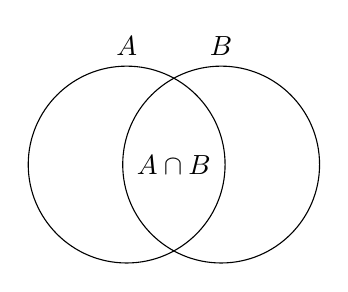
\begin{tikzpicture}

% Set A
\node [draw,circle,minimum size = 2.5cm,label={$A$}] (A) at (0,0){};

% Set B
\node [draw,circle,minimum size = 2.5cm,label={$B$}] (A) at (1.2,0){};

% Set intersection 
\node at (0.6,0) {$A \cap B$};

\end{tikzpicture}
\end{center}

O que acontece quando somamos os cardinais de $A$ e $B$ nessa situação? Isso mesmo, acabamos contando duplamente os elementos que estão na intersecção dos dois conjuntos. Para evitar essa dupla contagem, basta subtrairmos $|A \cap B|$\footnote{Ou seja, o cardinal da intersecção} da soma dos cardinais. A demonstração mais formal segue a baixo.

\begin{fact}[Fórmula da Inclusão-Exclusão para 2 conjuntos]
Se $A$ e $B$ são conjuntos finitos, então $|A \cup B| = |A| + |B| - |A \cap B|$.
\end{fact}

\begin{demonstration}
Se $A$ e $B$ são conjuntos, então teremos que:
\\
$$ |A \cup B| =  |A \cup (B - A)| = |A| + |(B-A)| $$
\\
Por outro lado, $(B-A)$ e $(A \cap B)$ também são conjuntos, cuja união é igual a:
\\
$$ |(B - A) \cup (A \cap B)| = |(B - A)| + |(A \cap B)| = |B|$$
\\
Apenas rearranjando essa segunda igualdade temos que,
\\
$$ |(B - A)| = |B| - |(A \cap B)| $$
\\
Substituindo o termo $|(B - A)|$ na primeira equação, 
\\
$$ |A \cup B| = |A| + |B| - |A \cap B| \ \blacksquare $$
\\
Essa demonstração foi inspirada nesse \href{https://people.maths.bris.ac.uk/~mb13434/incl_excl_n.pdf}{paper.}

\end{demonstration}

\textbf{Dica}: Tente resolver o exemplo 3.17 da página 93.
\\~\\
Claro que podemos nos deparar com situações que envolvam mais do que dois conjuntos. Para essas questões, vamos precisar de uma solução geral para $n$ conjuntos.

\begin{fact}[Fórmula da Inclusão-Exclusão]
Sejam $E_1$, $E_2$, $E_3$, ..., $E_n$ conjuntos quaisquer, então
\\~\\
$ |E_1 \cup E_2 \cup ... \cup E_n| = $
\begin{center}
$ + \left( \displaystyle \sum_{i = 1}^{n} |E_i| \right)$ \\
$ - \left( \displaystyle \sum_{1 \leq i < j \leq n} |E_i \cap E_j| \right) $ \\
$ + \left( \displaystyle \sum_{1 \leq i < j < k \leq n} |E_i \cap E_j \cap E_k | \right) $ \\
$ \vdots $ \\
\large $ (-1)^{n-1} |E_1 \cap E_2 \cap ... \cap E_n| $ 
\end{center}
\end{fact}

\begin{demonstration}
Partindo do caso caso mais simples, já sabemos que é verdade que, se $n = 1$ então $\displaystyle \bigcup_{i = 1}^{n} |A_i| =  \sum_{i = 1}^{n} |A_i|$. Agora vamos usar a \textbf{indução matemática}\footnote{Ainda vamos estudar mais pra frente sobre essa técnica, mas não é difícil entender o que ta rolando.} para demonstrar os casos onde temos $n + 1$.
\end{demonstration}


Suponha um elemento $x \in \bigcap_{i=1}^{n} A_{n}$, este será contado $n \choose 1$ no primeiro somatório.
$$\sum\limits_{i=1}^n |A_{n}|$$
$n \choose 2$ vezes no segundo:
$$\sum\limits_{1 \leq i<j \leq n} |A_{i} \cap A_{j}|$$
E assim por diante, o mesmo para o terceiro, pro quarto, etc.
\\
Como vimos anteriormente subtraímos a união entre $n$ conjuntos se $2|n$, isto é, $n$ é par, e somamos se $2 \nmid n$ e que ao fazermos isso garantimos que o elemento $x$ será contado um única vez. Portanto para garantirmos que isso temos que:
\begin{equation}
{n \choose 1} - {n \choose 2} +{n \choose 3} -{n \choose 4} ... + (-1)^{p-1} 
{n \choose p}
\end{equation}
\\
Como podemos garantir que essa fórmula resulta no que queremos? Bom, para isso precisamos lembrar de uma propriedade das combinações onde ${n \choose k} = {n \choose n-k}$. Isso implicaria que se fizermos ${n \choose 0} - (3.1) = 0$, está correto pois sabemos que ${n \choose 0} = 1$. Assim, está provado o Princípio da Inclusão-Exclusão, caso queira pode fazer prova por PIF.

\section{Contando Multiconjuntos}
No decorrer deste capítulo já aprendemos muitas coisas, Combinações, Arranjos, Permutações, etc. Porém como pode passar em sua cabeça ainda não sabemos trabalhar com elementos repetidos nos conjuntos, sim, sabemos que conjuntos não permitem repetições. Portanto é necessário introduzir um novo elemento da matemática, os \textbf{multiconjuntos.}
\\~\\
Nos multiconjuntos as repetições são permitidas e a ordem com que os elementos estão dispostos dentro dele não importa tal qual nos conjuntos. Isso faz deles um híbrido entre conjuntos e listas.
\\~\\
Dos conjuntos ainda conserva-se uma propriedade, a \textbf{cardinaldiade}, a ideia é exatamente a mesma, a cardinalidade é a quantidade de elementos do multiconjuntos. A outra propriedade dos multiconjuntos é a \textbf{multiplicidade}, esta por sua vez é a quantidade de vezes que um elemento qualquer repete-se dentro do multiconjuntos.

\begin{fact}[Contagem de Multiconjuntos]
Sejam $x_{1}, x_{2}, x_{3},... x_{n}$ a multiplicidade de cada um dos $n$ elementos do multiconjuntos $A$, o número total de permutações possíveis é dado por:
$$\frac{n!}{x_{1}!x_{2}!...x_{n}!}$$
\end{fact}
Com a boa compreensão que temos da contagem de subconjuntos esse parte fica muito fácil de ser compreendida porque o mecanismo é exatamente o mesmo.
\\~\\
Temos um multiconjuntos de $n$ elementos. Portanto, ignorando os elementos repetidos, o número de permutações que temos desse multiconjuntos é $n! = n(n-1)...(n-n)!$.
\\~\\
Lembre-se do que fizemos na parte contagem de subconjuntos, nós eliminamos conjuntos que "davam na mesma" dividindo a fórmula da combinação pela cardinalidade dos subconjuntos, faremos algo bem semelhante aqui.
\\~\\
Vamos usar a palavra "banana" como exemplo, se ignorarmos os que "a" repete-se três vezes e "n" repete-se duas vezes, então o número de combinação possíveis são $6! = 720$. Agora vamos fixar as letras "b" e "a" e permutar apenas as letras "n" então teremos:
\begin{center}
BA\textit{N}ANA\\
BANA\textit{N}A
\end{center}
Obviamente permanecem a mesma palavra mesmo trocando "N" de lugar, e o número de palavras que permanecem iguais é o fatorial da cardinalidade de "N" dentro do multiconjunto. Agora pense se realmente permutássemos todo o multiconjunto, nós teríamos sempre essas duas combinações somente com ambos os N's mudando de lugar, portanto podemos dividir $6!$ pela cardinalidade de "N" que no caso é $2$.
\\~\\
Agora vamos fazer o mesmo com a letra "A" (vou tentar deixar mais fácil de identificá-los nas combinações):
\begin{center}
BA$_{1}$NA$_{2}$NA$_{3}$ \\
BA$_{1}$NA$_{3}$NA$_{2}$ \\
BA$_{2}$NA$_{1}$NA$_{3}$ \\
BA$_{2}$NA$_{3}$NA$_{1}$ \\
BA$_{3}$NA$_{1}$NA$_{2}$ \\
BA$_{3}$NA$_{2}$NA$_{1}$ \\
\end{center}
E novamente seguimos a mesma lógica, para as várias combinações da palavra "banana" teremos o fatorial da multiplicidade de "A" em palavras que dão na mesmo, então podemos dividir $6!$ por $3!$, para eliminar as palavras iguais.
\\~\\
Porém já sabemos que o número de permutações não é $6!$, mas sim $\frac{6!}{2!}$, agora é só dividir isso por $3!$, então, $\frac{6!}{2!3!}$.
\\~\\
Agora o \textbf{Fato 3.8.1} ficou bem mais intuitivo.

\section{Os Princípios da Divisão e da Casa dos Pombos}

Estamos chegando ao fim de nossa caminhada pelos fundamentos matemático do nosso curso faltam apenas mais alguns conceitos em nossa bagagem matemática para seguirmos adiante, um deles é o \textbf{Princípio da Divisão}.
\\~\\
Para isso é preciso introduzir uma nova notação, $\lfloor x \rfloor$ é o \textit{floor} (vou manter o termo em inglês) é o número inteiro menor que $x$ mais próximo $x$. E $\lceil x \rceil$ é o \textit{ceiling}, ou seja, o número inteiro maior que $x$ mais próximo de $x$.
\\~\\
Agora imagine que você pussui 15 bolinhas e 10 recipientes e queira dispô-las dentro de cada recipiente, quantas bolinhas cada recipiente terá? Bem, podemos simplesmente dividir o número de bolinhas pelo número de recipientes, $\frac{15}{10} = 1,5$. Ok, isso não está completamente errado, mas pelo menos da forma que estamos trabalhando não temos $0,5$ bolinhas, esse valor é a média de bolinhas por recipiente, isso quer dizer que na verdade cada recipiente possui pelo menos uma. Disso segue: 
\begin{fact}[O Princípio da Divisão]
Suponha $n$ objetos dispostos em $k$ caixas. \\
Então pelo menos uma caixa possui $\lceil \frac{n}{k} \rceil$ objetos ou mais, e
pelo menos uma caixa possui $\lfloor \frac{n}{k} \rfloor$ objetos ou menos.
\end{fact}
Agora suponha $n$ pombos que ao final da tarde voam de volta para seu viveiro onde existem $k$ casinhas, o que ocorre se $n > k$ ou $n < k$?
No primeiro caso $\frac{n}{k} > 1$, isso é, existe pelo menos uma casinha que possui mais que um pombo, no segundo caso $\frac{n}{k} < 1$ o que significa que ao menos uma casinha está vazia. Disso surge:
\begin{fact}[O Princípio da Casa dos Pombos]
Suponha $n$ objetos dispostos em $k$ caixas.\\
Se $n > k$, então pelo menos uma caixa possui mais que dois objetos.\\
Se $n < k$, então pelo menos uma caixa está vazia.
\end{fact}
Sabemos que parece bobo ter que definir isso, mas o próprio Hammack dá uma boa explicação que não tiraríamos uma única vírgula:
\begin{quote}
Like the multiplication, addition and subtraction principles, the division
and pigeonhole principles are intuitive and obvious, but they can prove
things that are not obvious. The challenge is seeing where and how to apply
them. \footnote{Tradução: "Como os princípios da multiplicação, adição e subtração, o princípio da divisão e da casa dos pombos são intuitivos e obvios, mas eles podem provar coisas que não são obvias. O desafio é ver onde e como aplicá-los."}
\end{quote}

\section{Prova Combinatorial}
No decorrer desse capítulo provamos diversas relações combinatoriais como:
$$ {n+1 \choose k} = {n \choose k-a} + {n \choose k}$$
$${n \choose n-k} = {n \choose k}$$

Porém existem outras relações interessantes que ainda podemos provar por aqui, por exemplo:
$$\sum_{k = 0}^{n} {n \choose k}^2 = {2n \choose n}$$
\\
Suponha um conjuntos $S = A \cup B, \ A \cap B = \emptyset$ e $|S| = 2n$, se quiser combinar seus elementos $n$ a $n$ pode selecionar $k$ elementos de $A$ e $n-k$ de $B$, pois $k+(n-k) = n$, então pelo \textbf{Princípio da Multiplicação} ${n \choose k}{n \choose n-k}$. Como $0 \leq k \leq n$, temos que:
$${2n \choose n} = \underbrace{n \choose 0}_{0 \ de \ A}\underbrace{n \choose n}_{n \ de \ B} + \underbrace{n \choose 1}_{1 \ de \ A}\underbrace{n \choose n-1}_{n-1 \ de \ B} + \dots + \underbrace{n \choose n}_{n \ de \ A}\underbrace{n \choose 0}_{0 \ de \ B}$$
Sabemos que ${n \choose k} = {n \choose n-k}$, teremos:
$${2n \choose n} = {n \choose 0}^2 + {n \choose 1}^2 + \dots {n \choose n}^2 = \sum_{k = 0}^{n} {n \choose k}^2 \blacksquare$$
%%%%%%%%%%%%%%%%%%%%%%%%%%%%%%%%%%%%%%%%%%%%%%%%%%%
%                    PART                         %
%%%%%%%%%%%%%%%%%%%%%%%%%%%%%%%%%%%%%%%%%%%%%%%%%%%
\end{document}
